\chapter{Test Jezelf}

In de loop van het academiejaar leg je voor dit vak drie testen af. Deze testen tellen mee voor 40\% van het eindtotaal en vormen dus een bijzonder belangrijk deel van je eindscore! Het wordt dan ook zeer hard aangeraden om deze testen  goed voor te bereiden. Om je hierbij te helpen hebben we in dit hoofdstuk een aantal testen en examens van een vorig academiejaar gebundeld, zodat je weet waar je je aan kan verwachten.

Alle testen volgen elkaar direct op. Let dus goed op welke bladzijden bij welke test horen (kijk naar de nummering van de vragen en de hoofding van de test)!

Dit hoofdstuk bevat (in deze volgorde):

\begin{itemize}
\item drie testen over `Controlestructuren'
\item drie testen over `Recursie'
\item drie testen over `Arrays'
\item twee examens
\end{itemize}

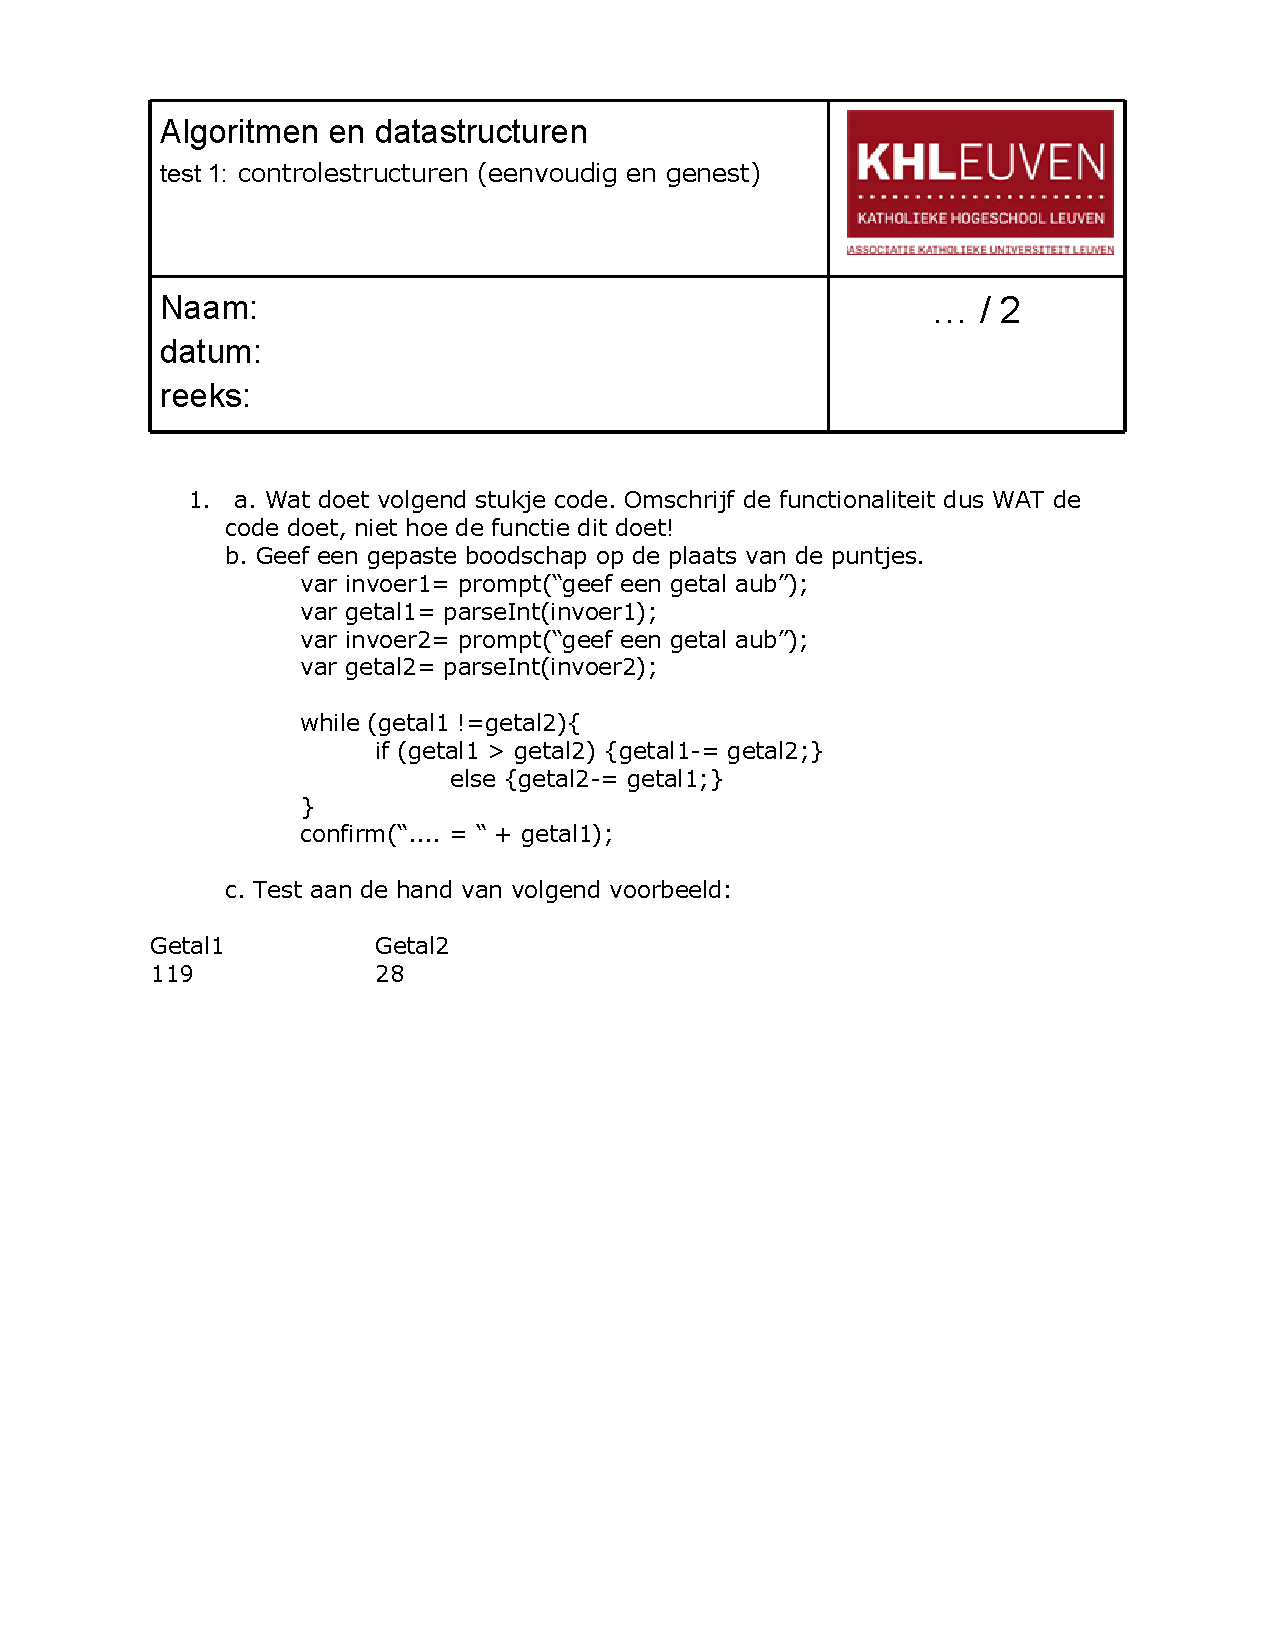
\includepdf[pages={-}]{Testen/Controlestructuren1.pdf}
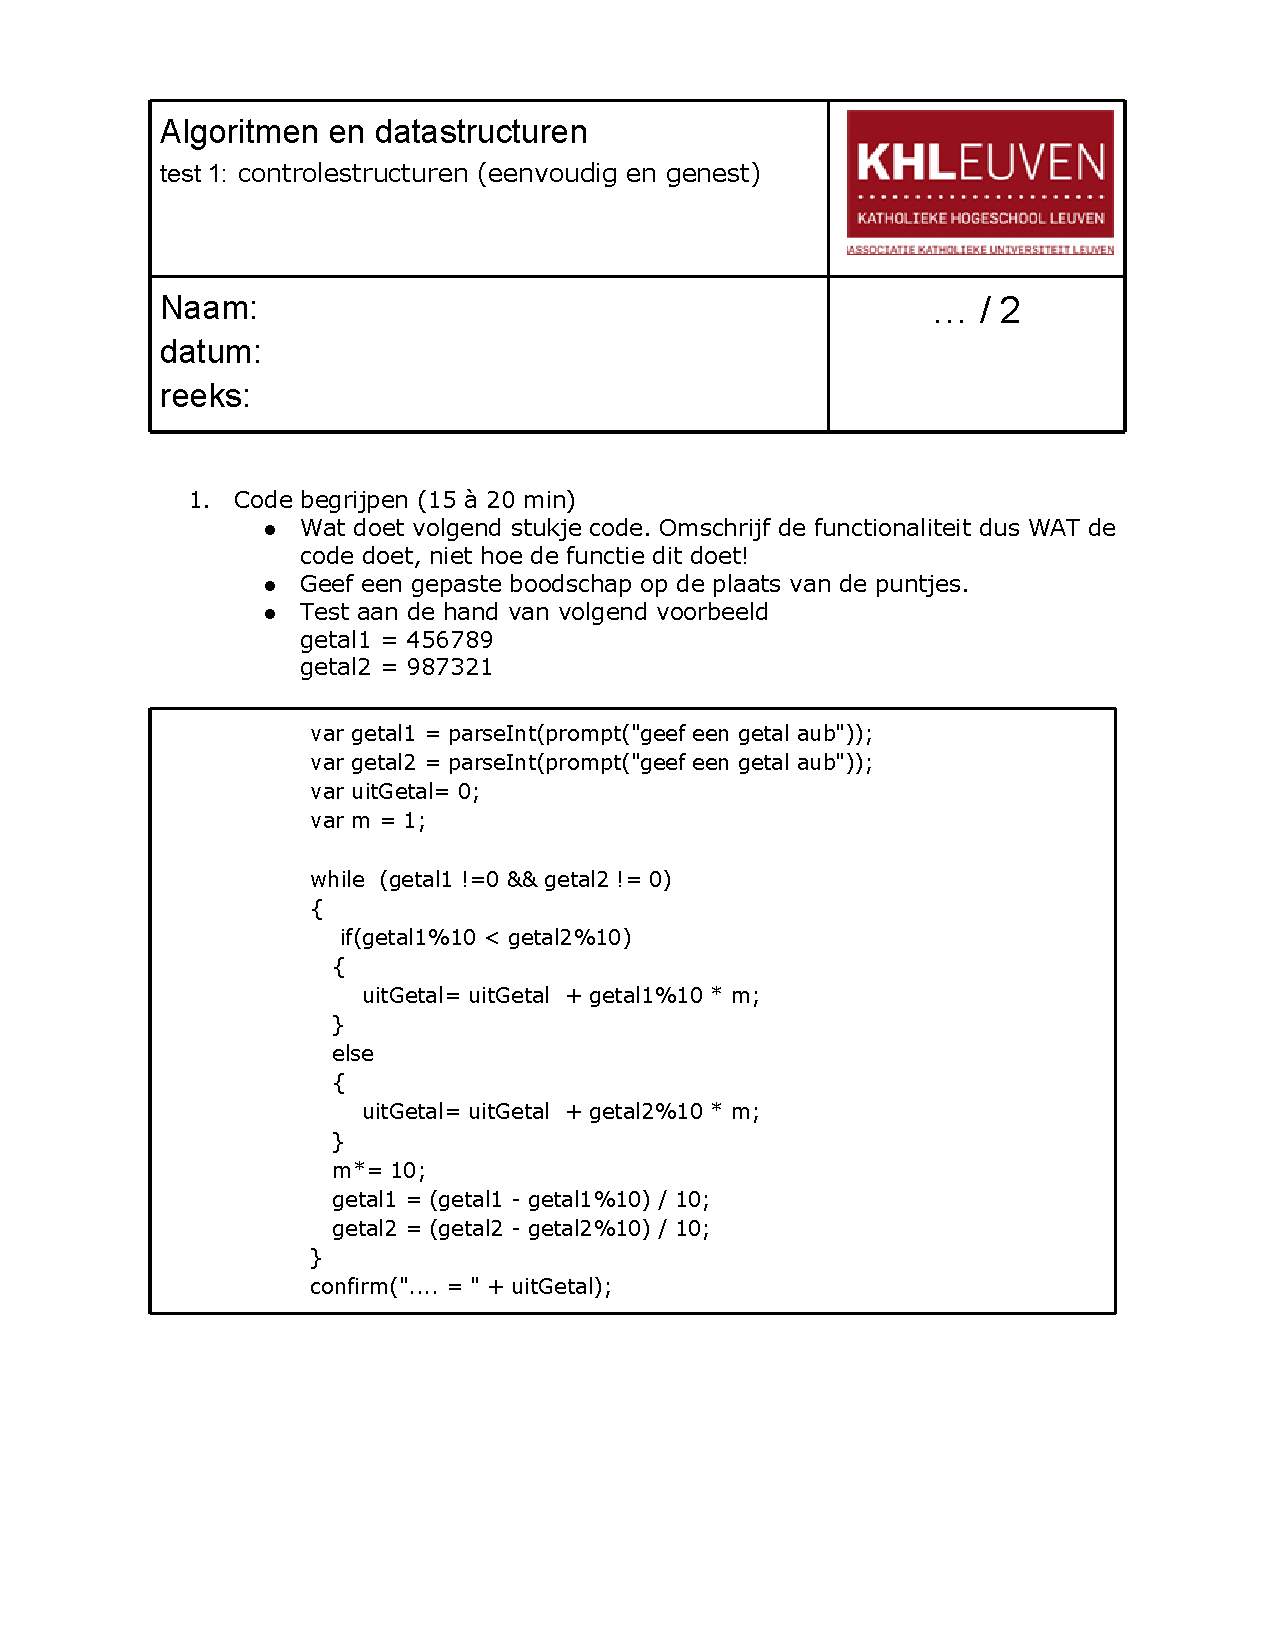
\includepdf[pages={-}]{Testen/Controlestructuren2.pdf}
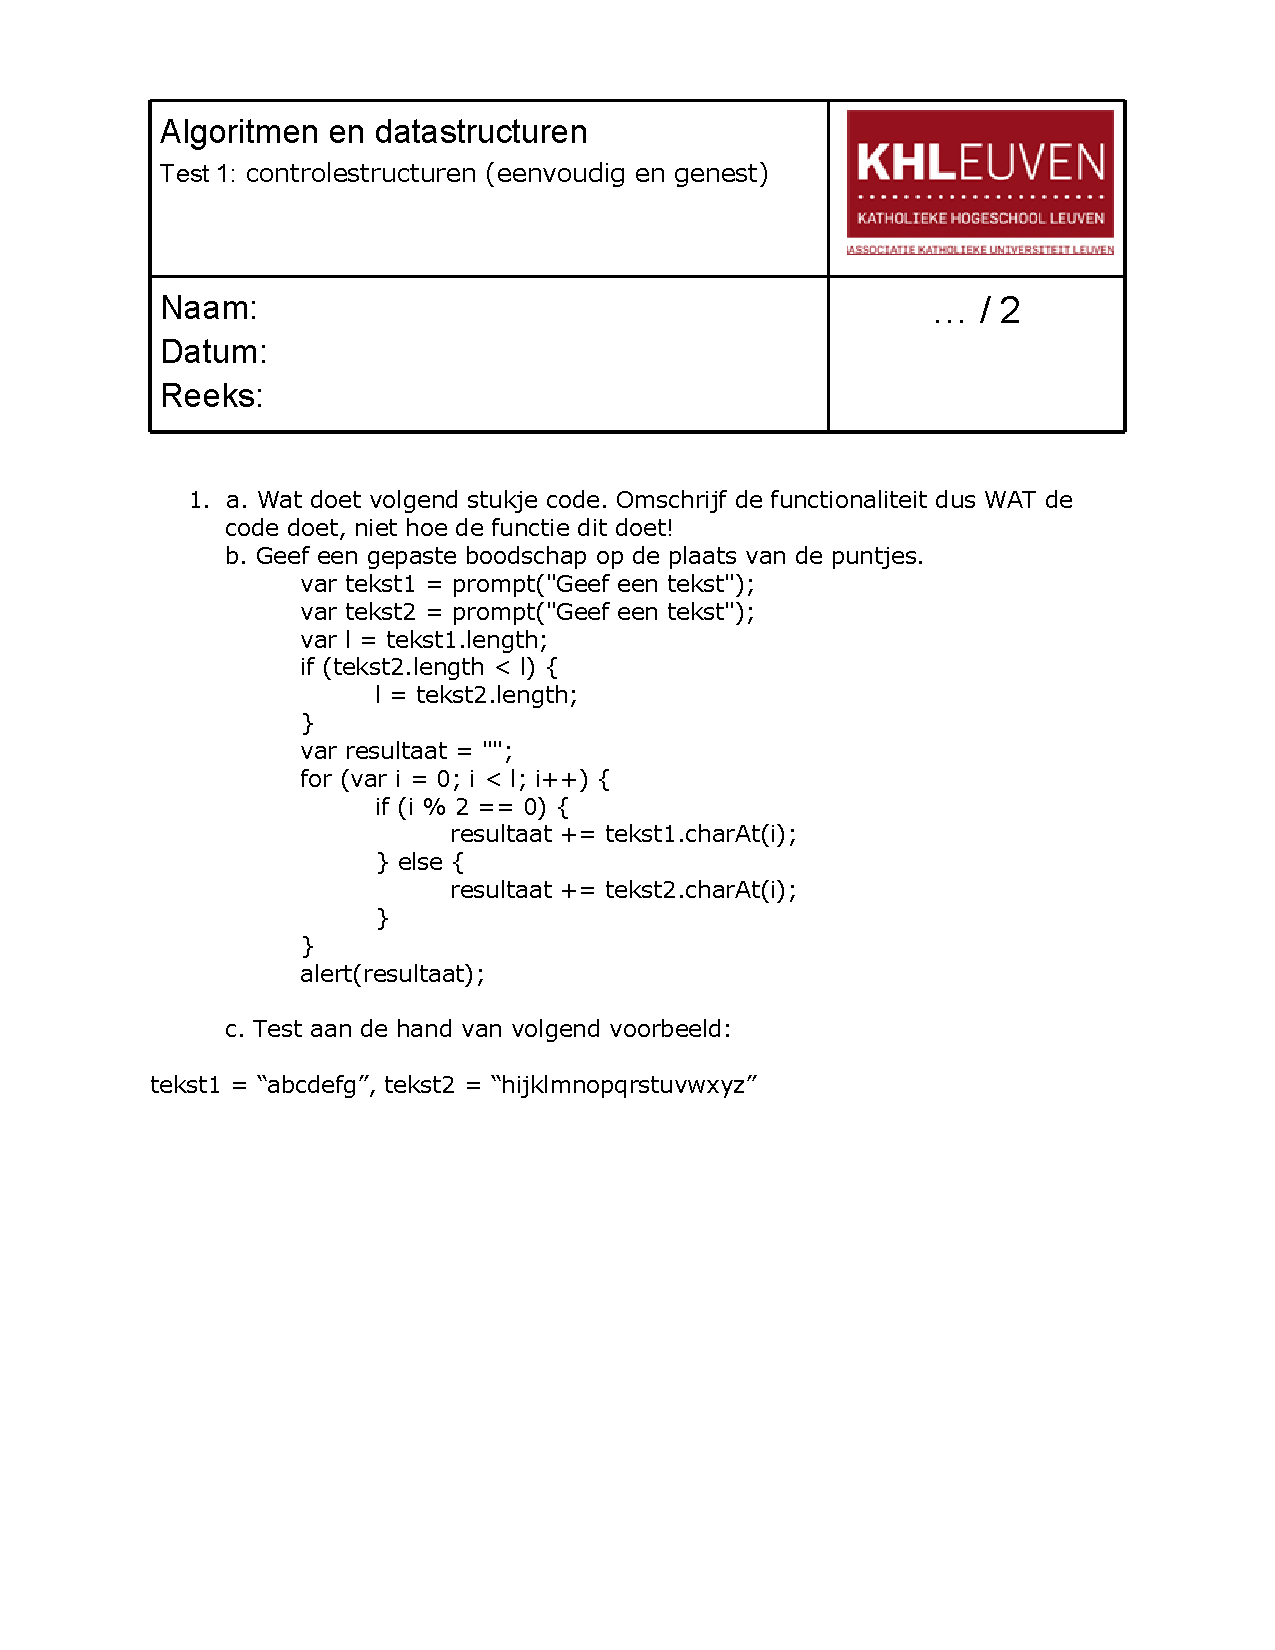
\includepdf[pages={-}]{Testen/Controlestructuren3.pdf}

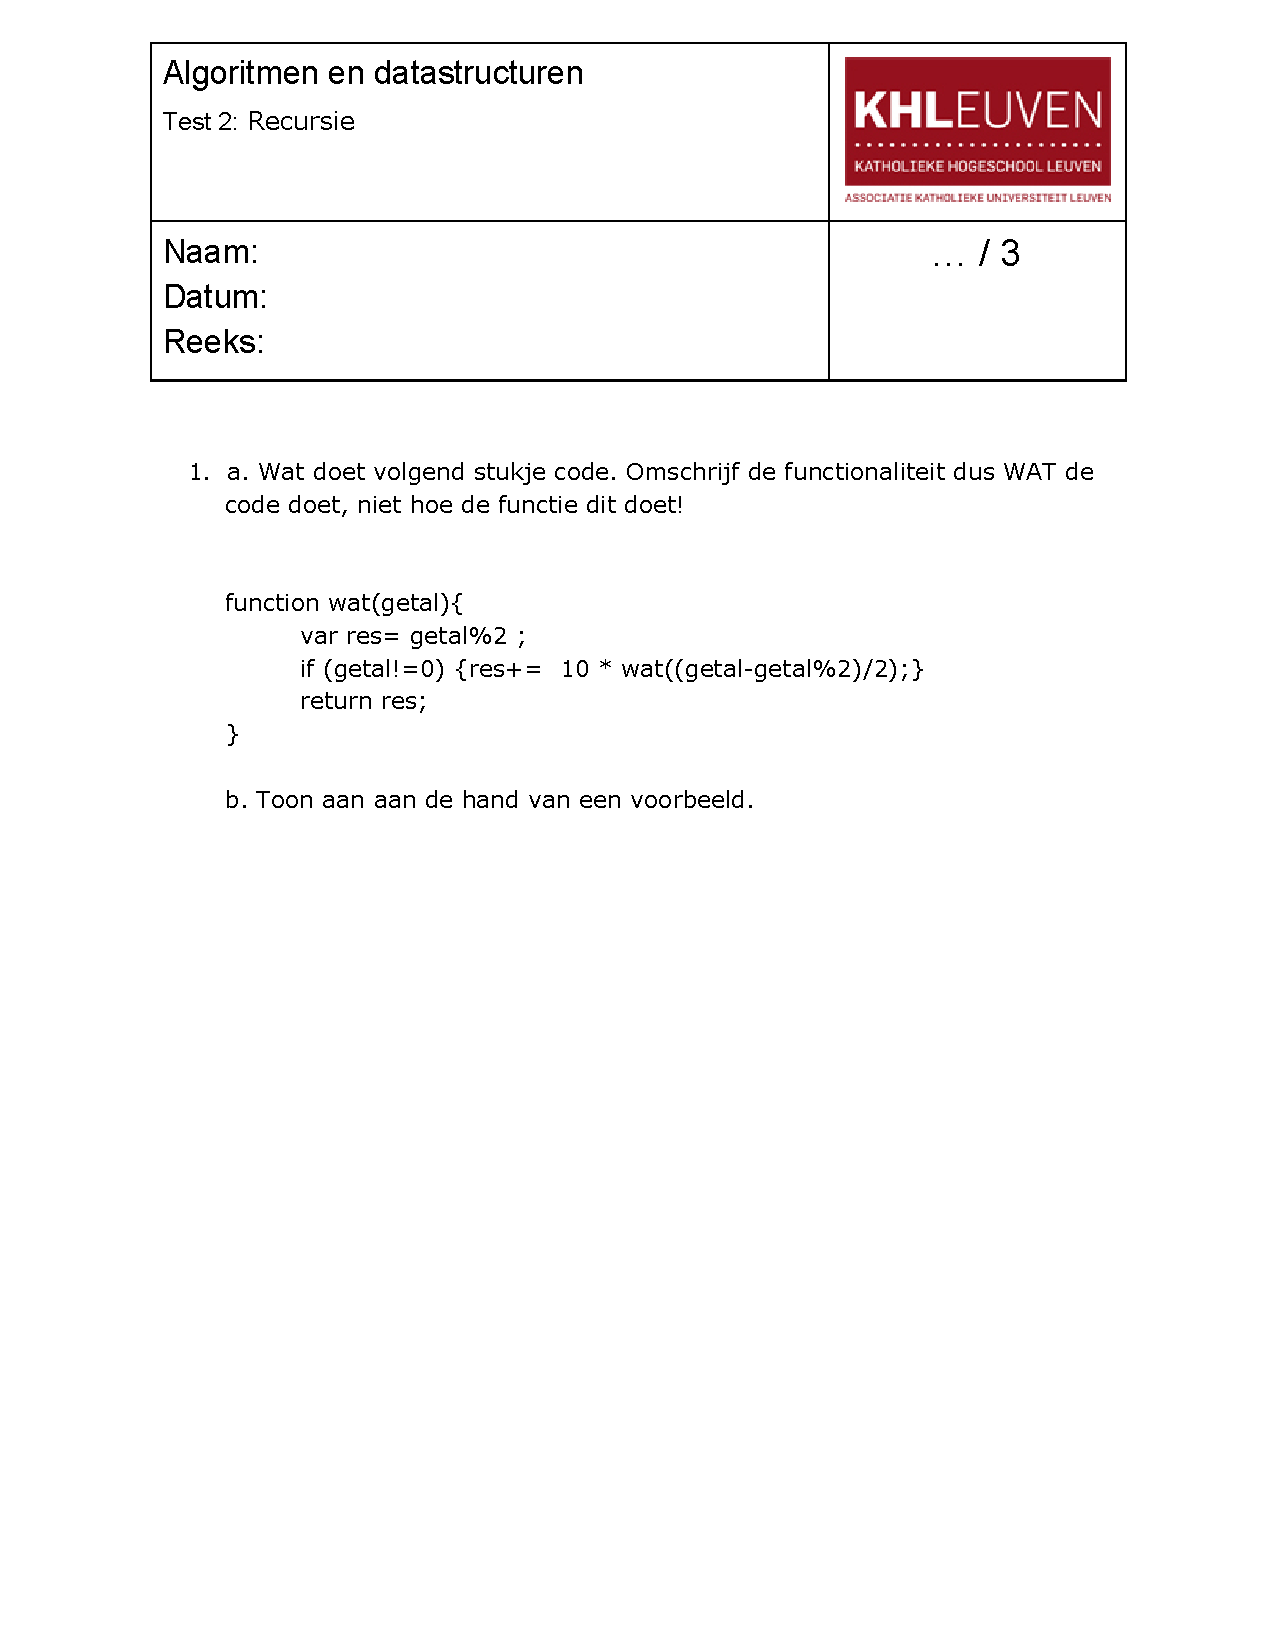
\includepdf[pages={-}]{Testen/Recursie1.pdf}
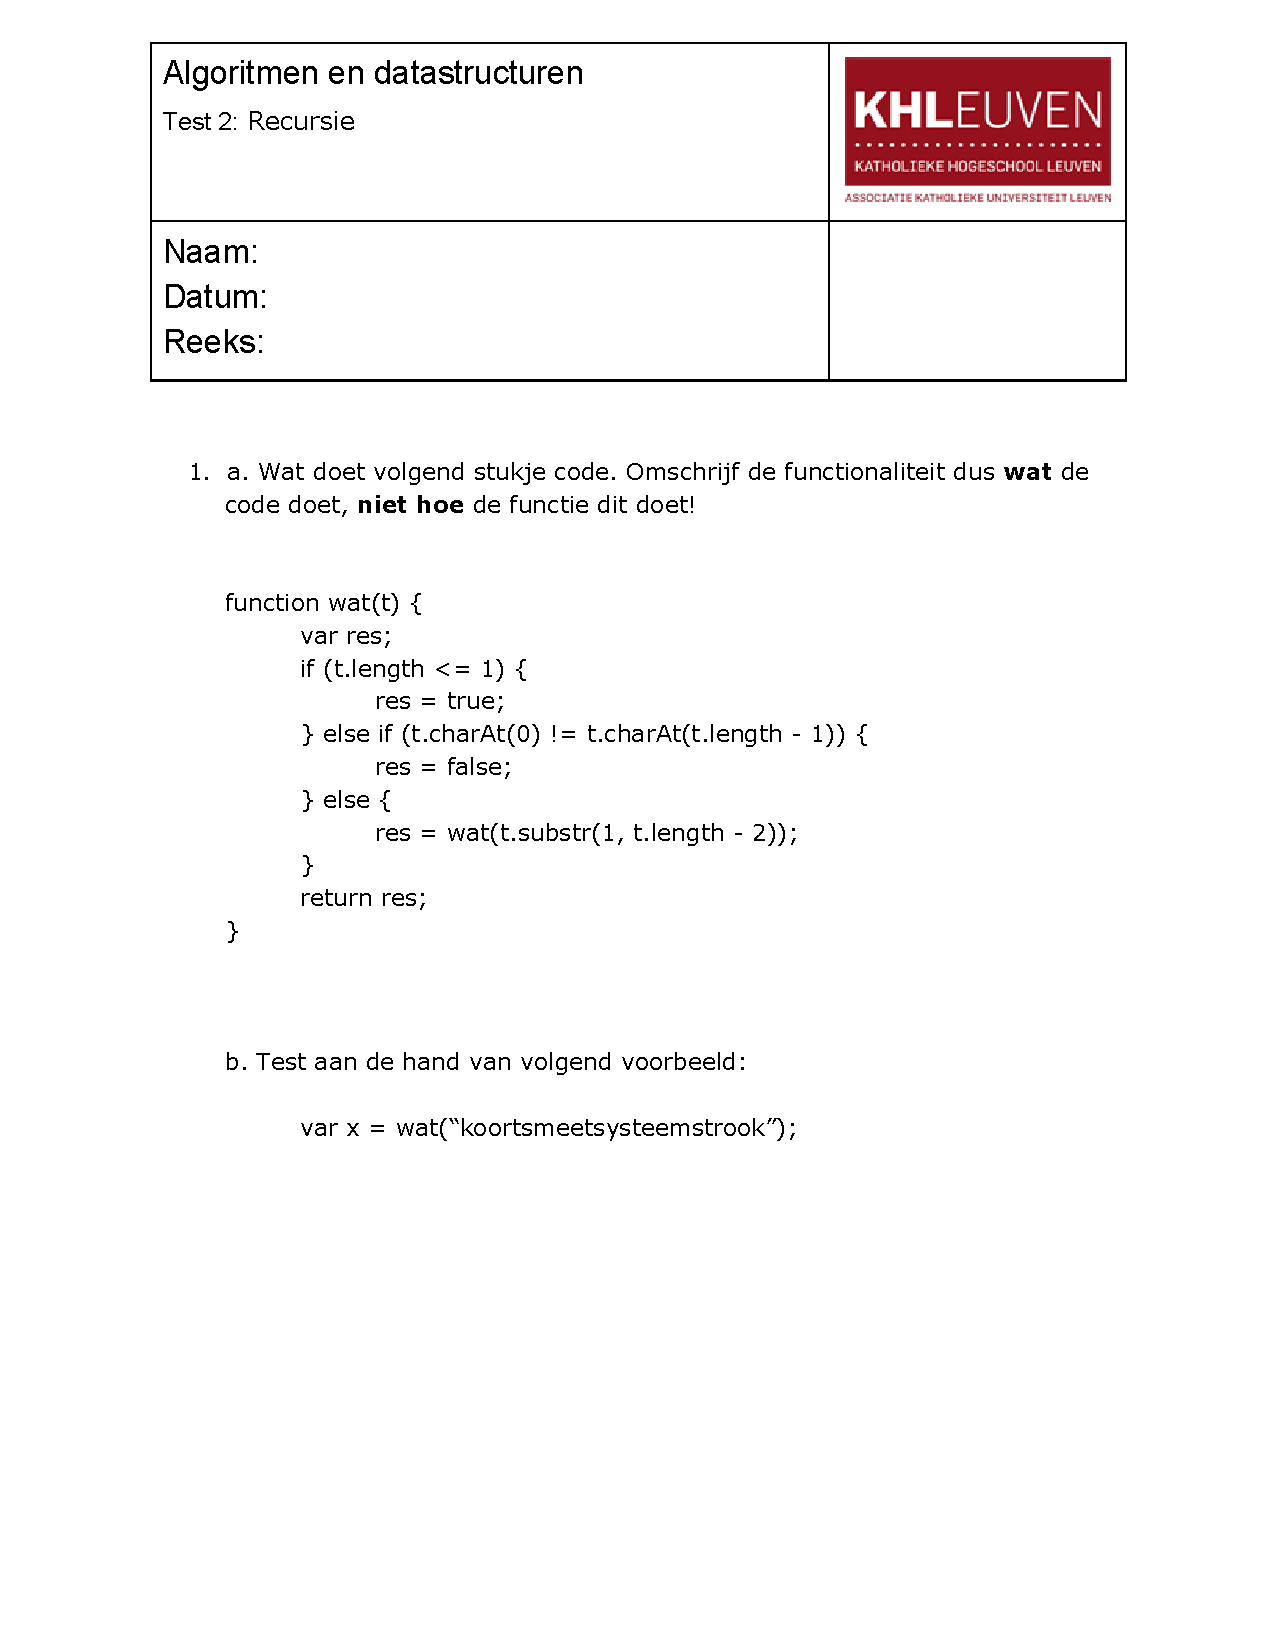
\includepdf[pages={-}]{Testen/Recursie2.pdf}
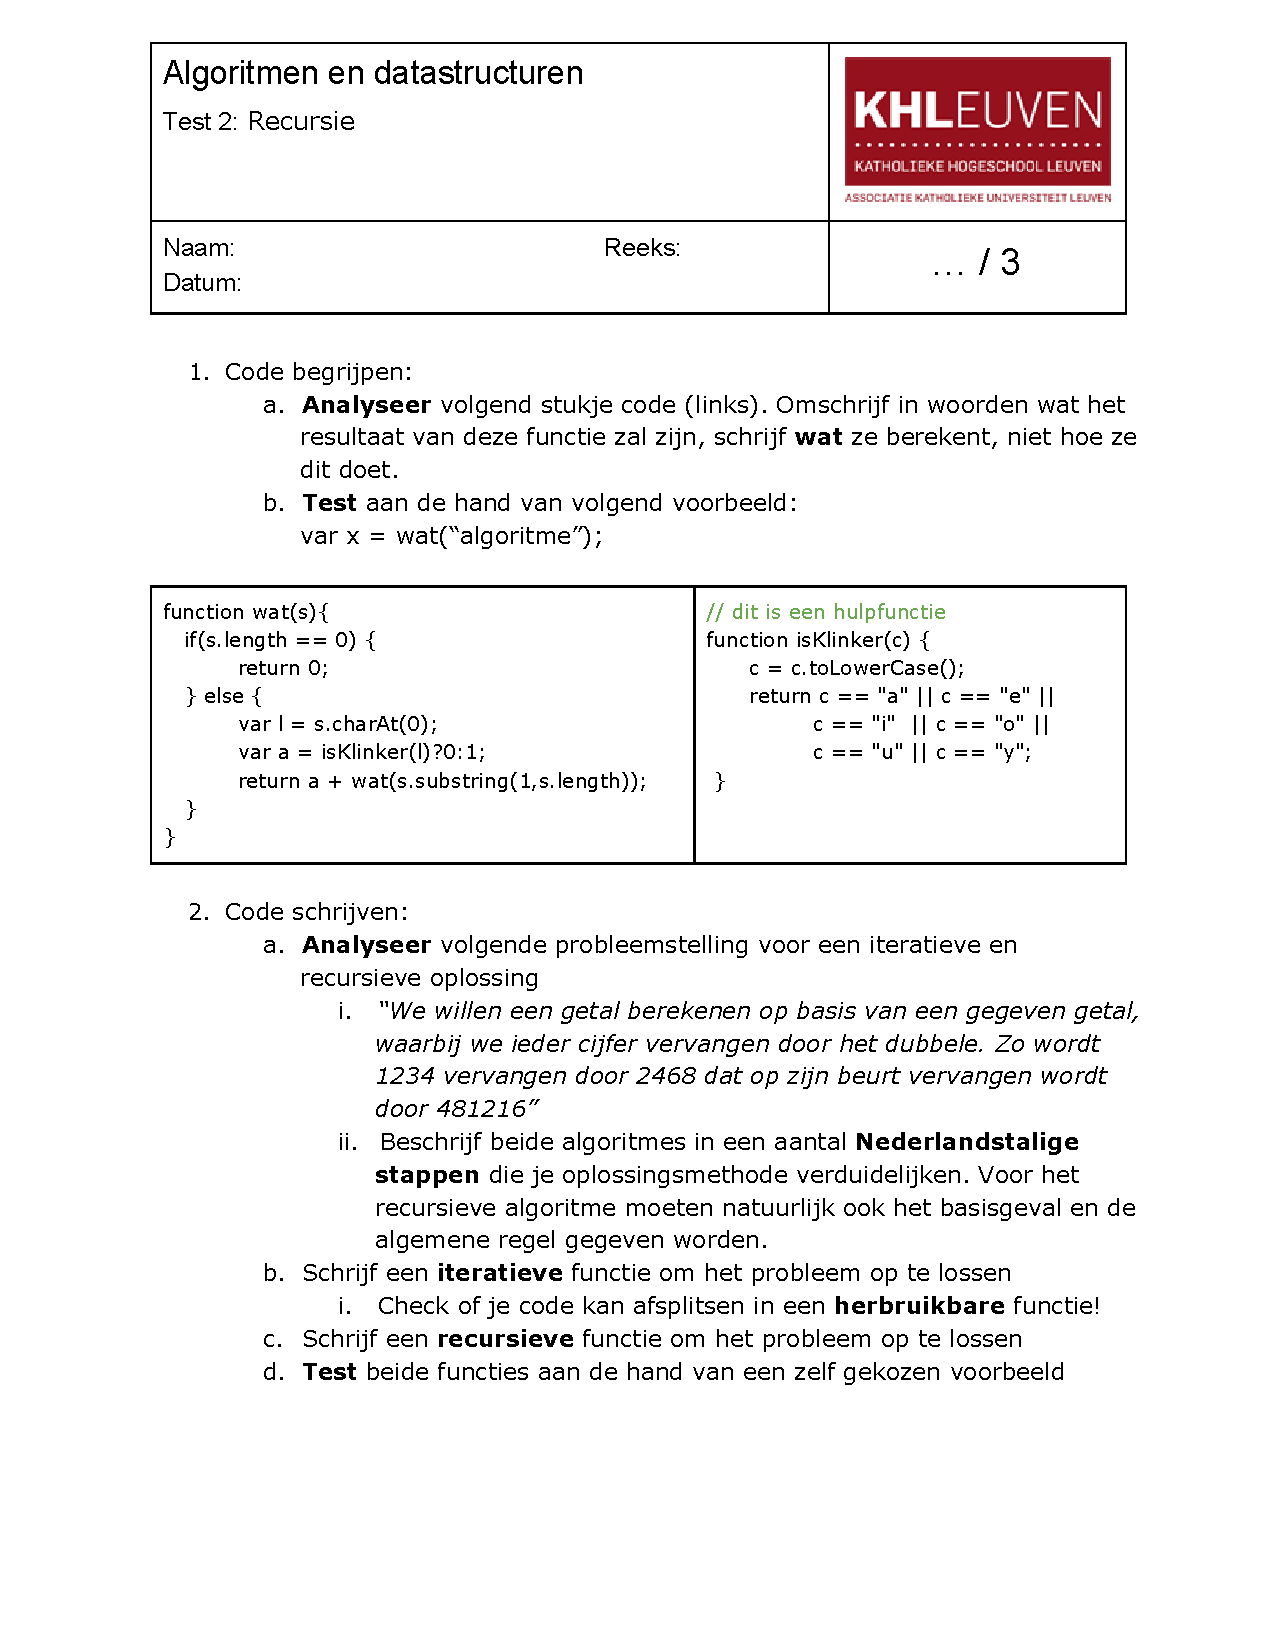
\includepdf[pages={-}]{Testen/Recursie3.pdf}

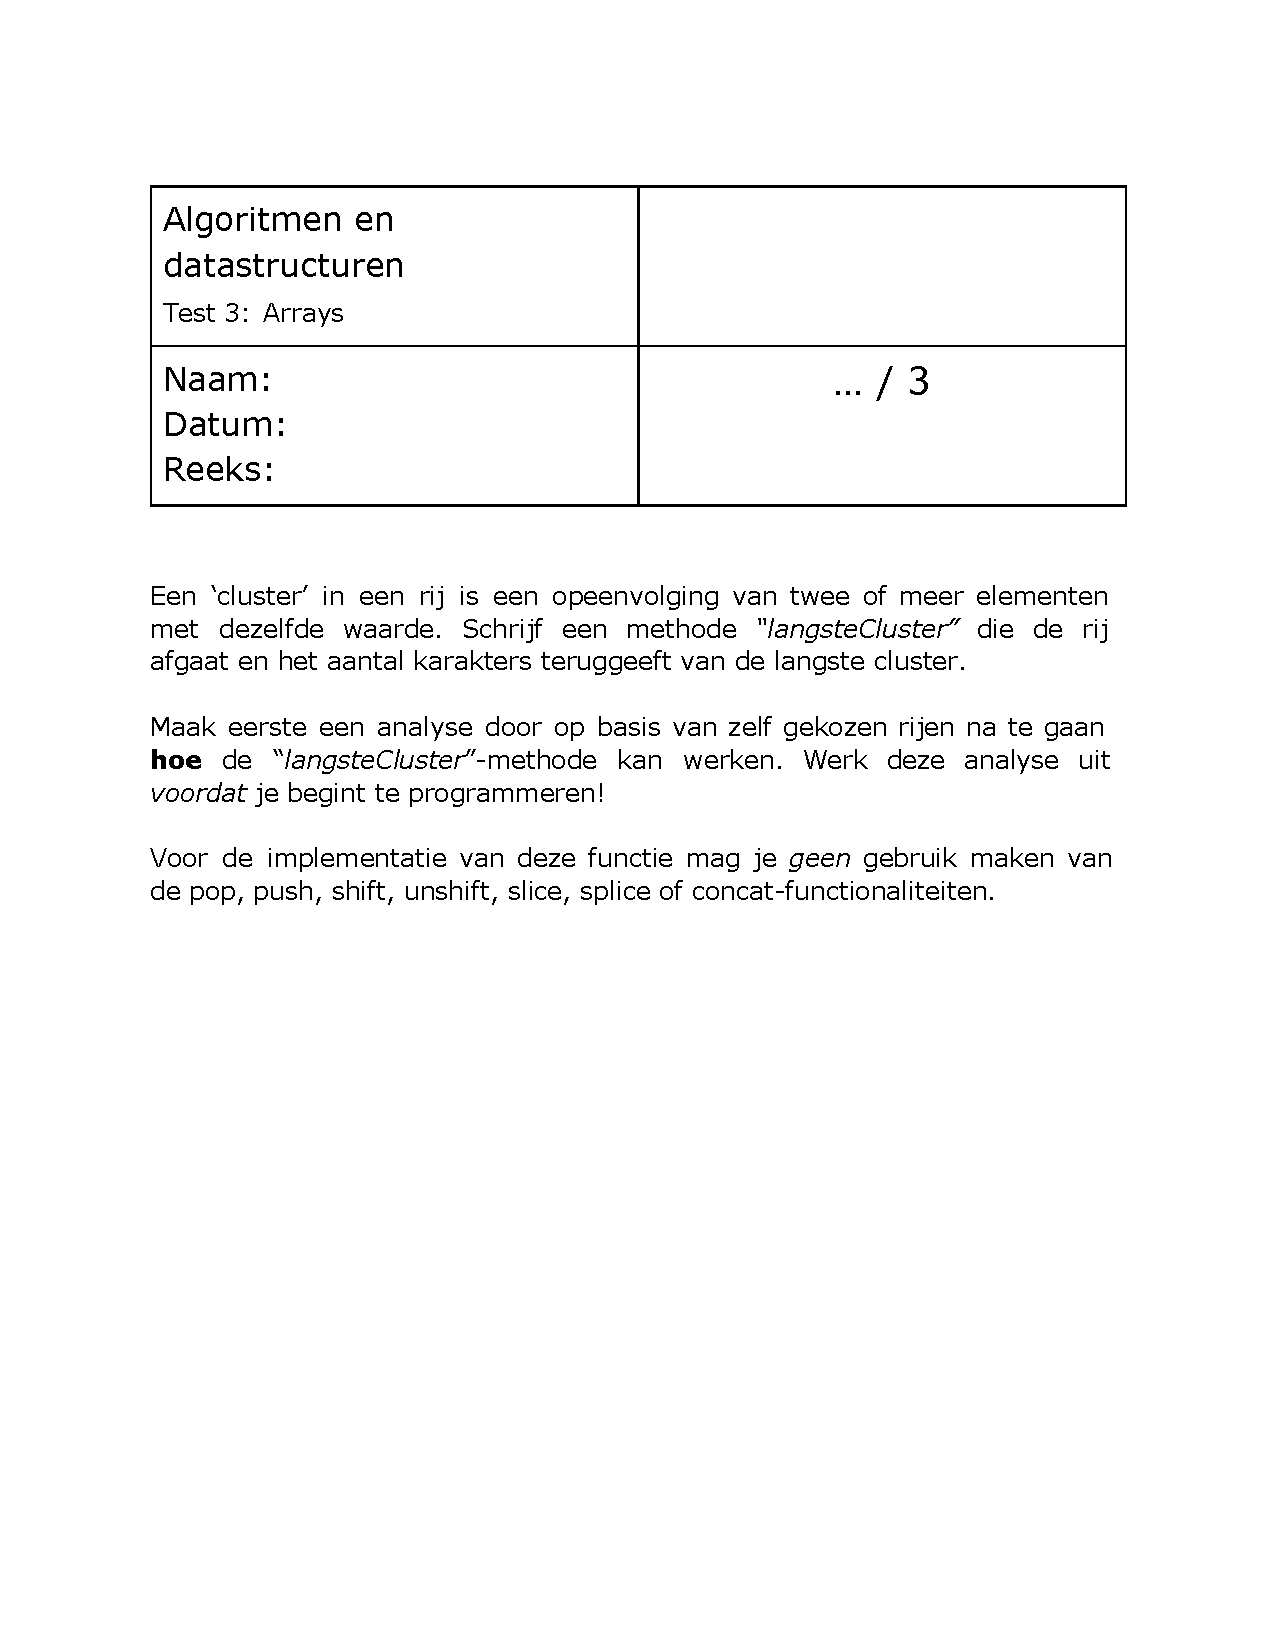
\includepdf[pages={-}]{Testen/Arrays1.pdf}
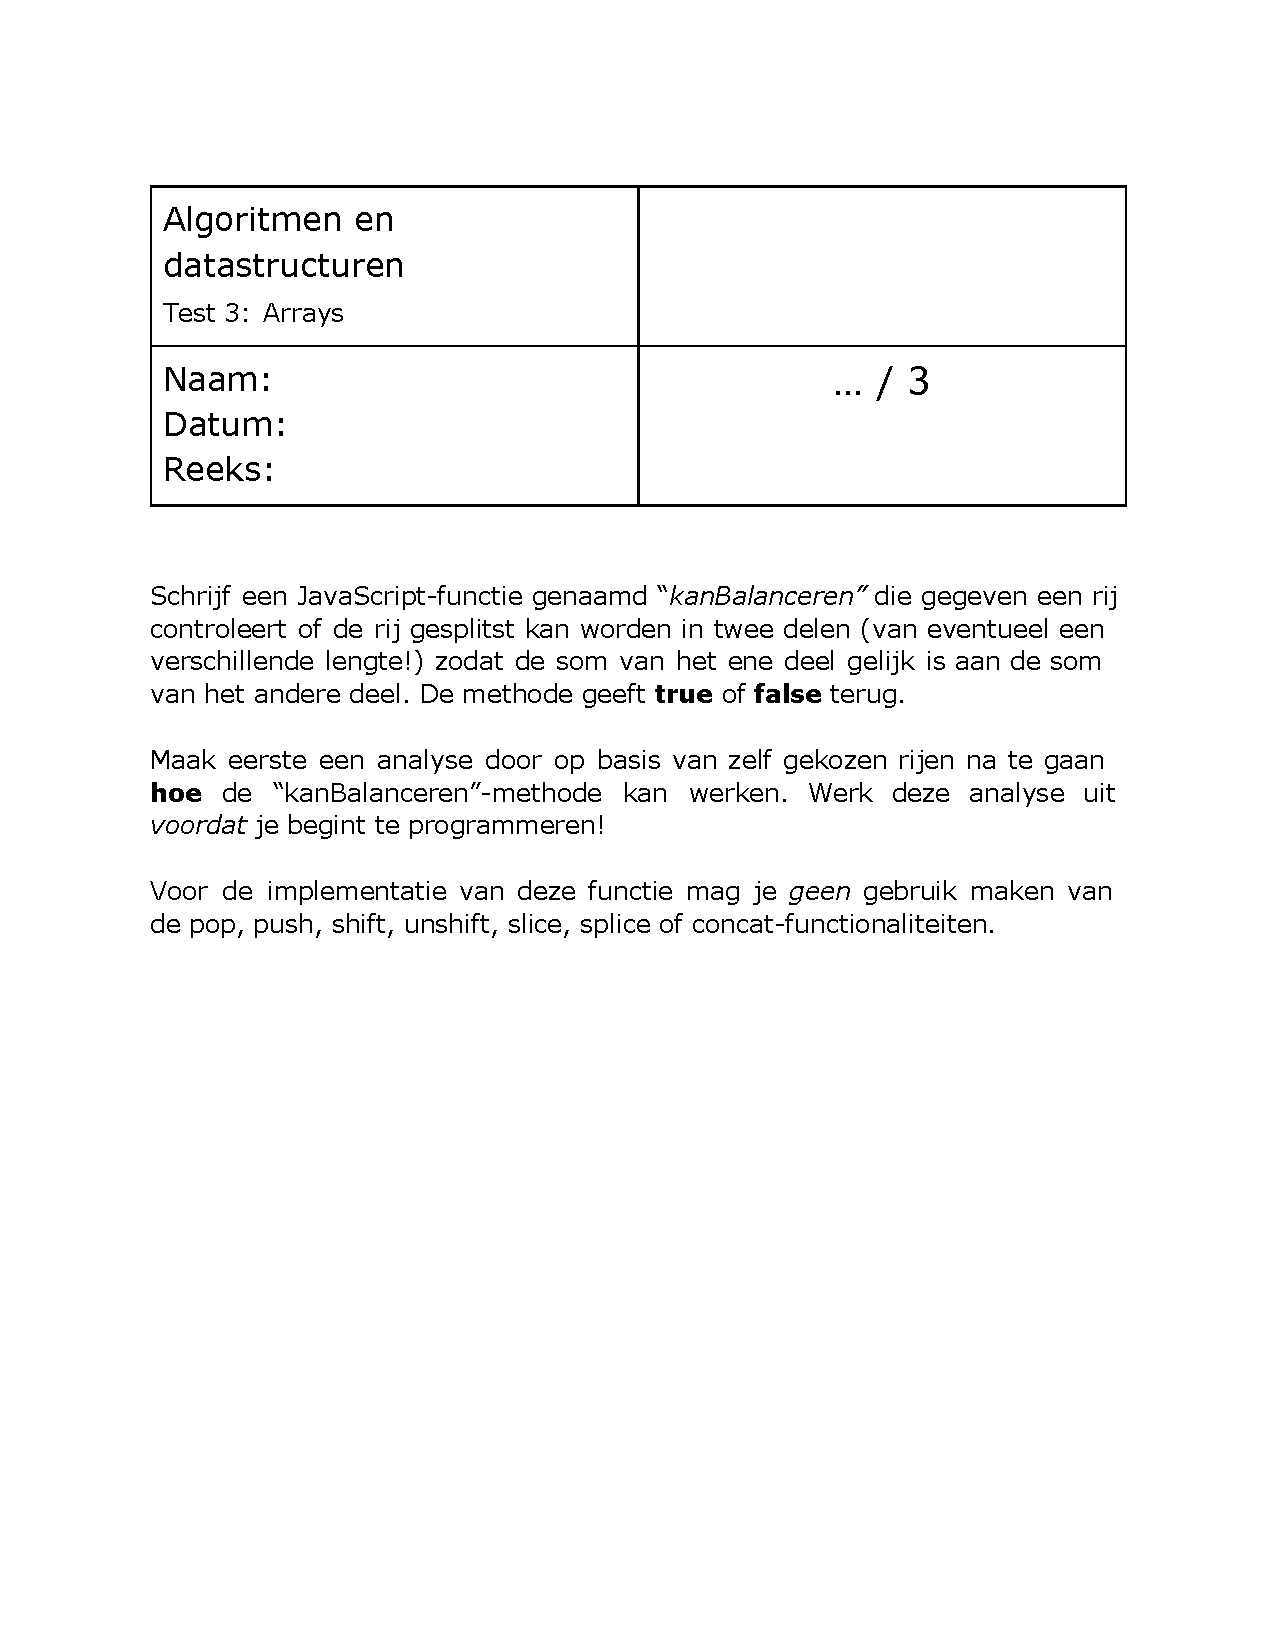
\includepdf[pages={-}]{Testen/Arrays2.pdf}
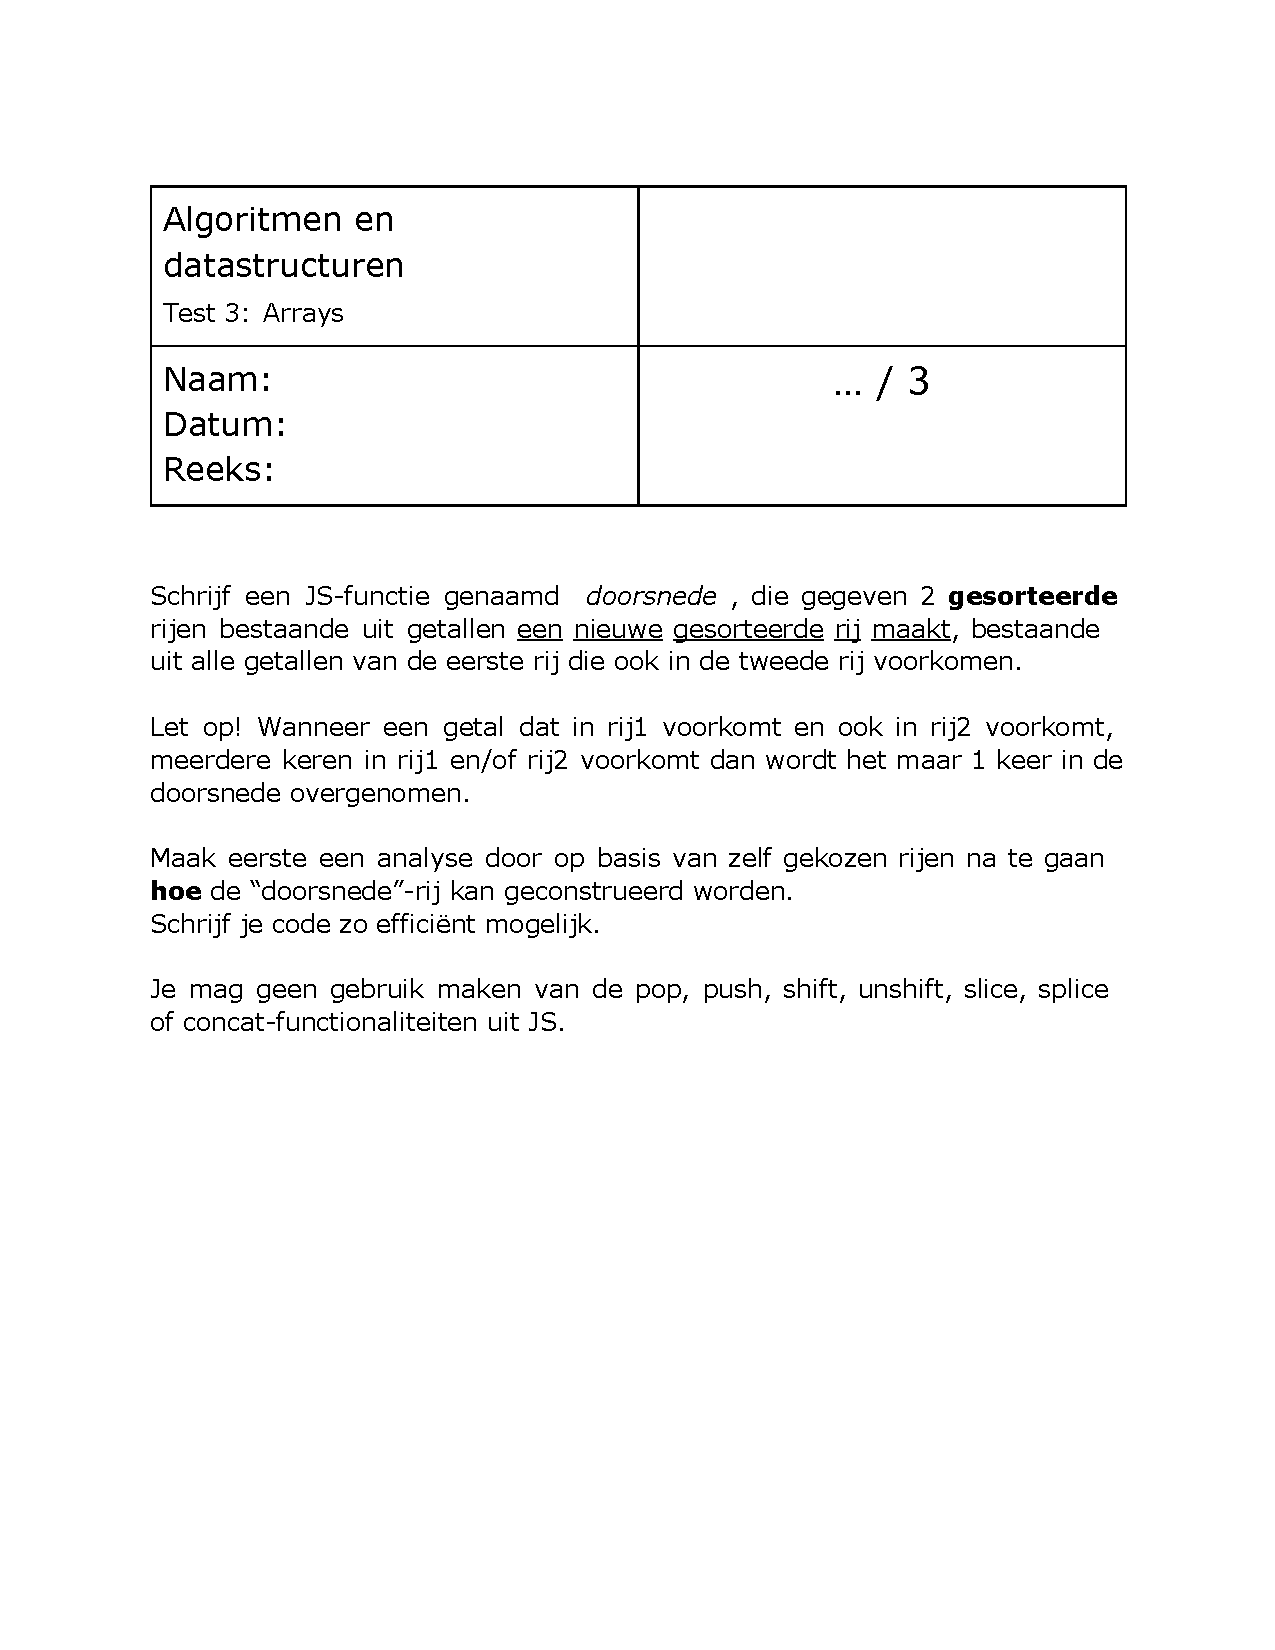
\includepdf[pages={-}]{Testen/Arrays3.pdf}

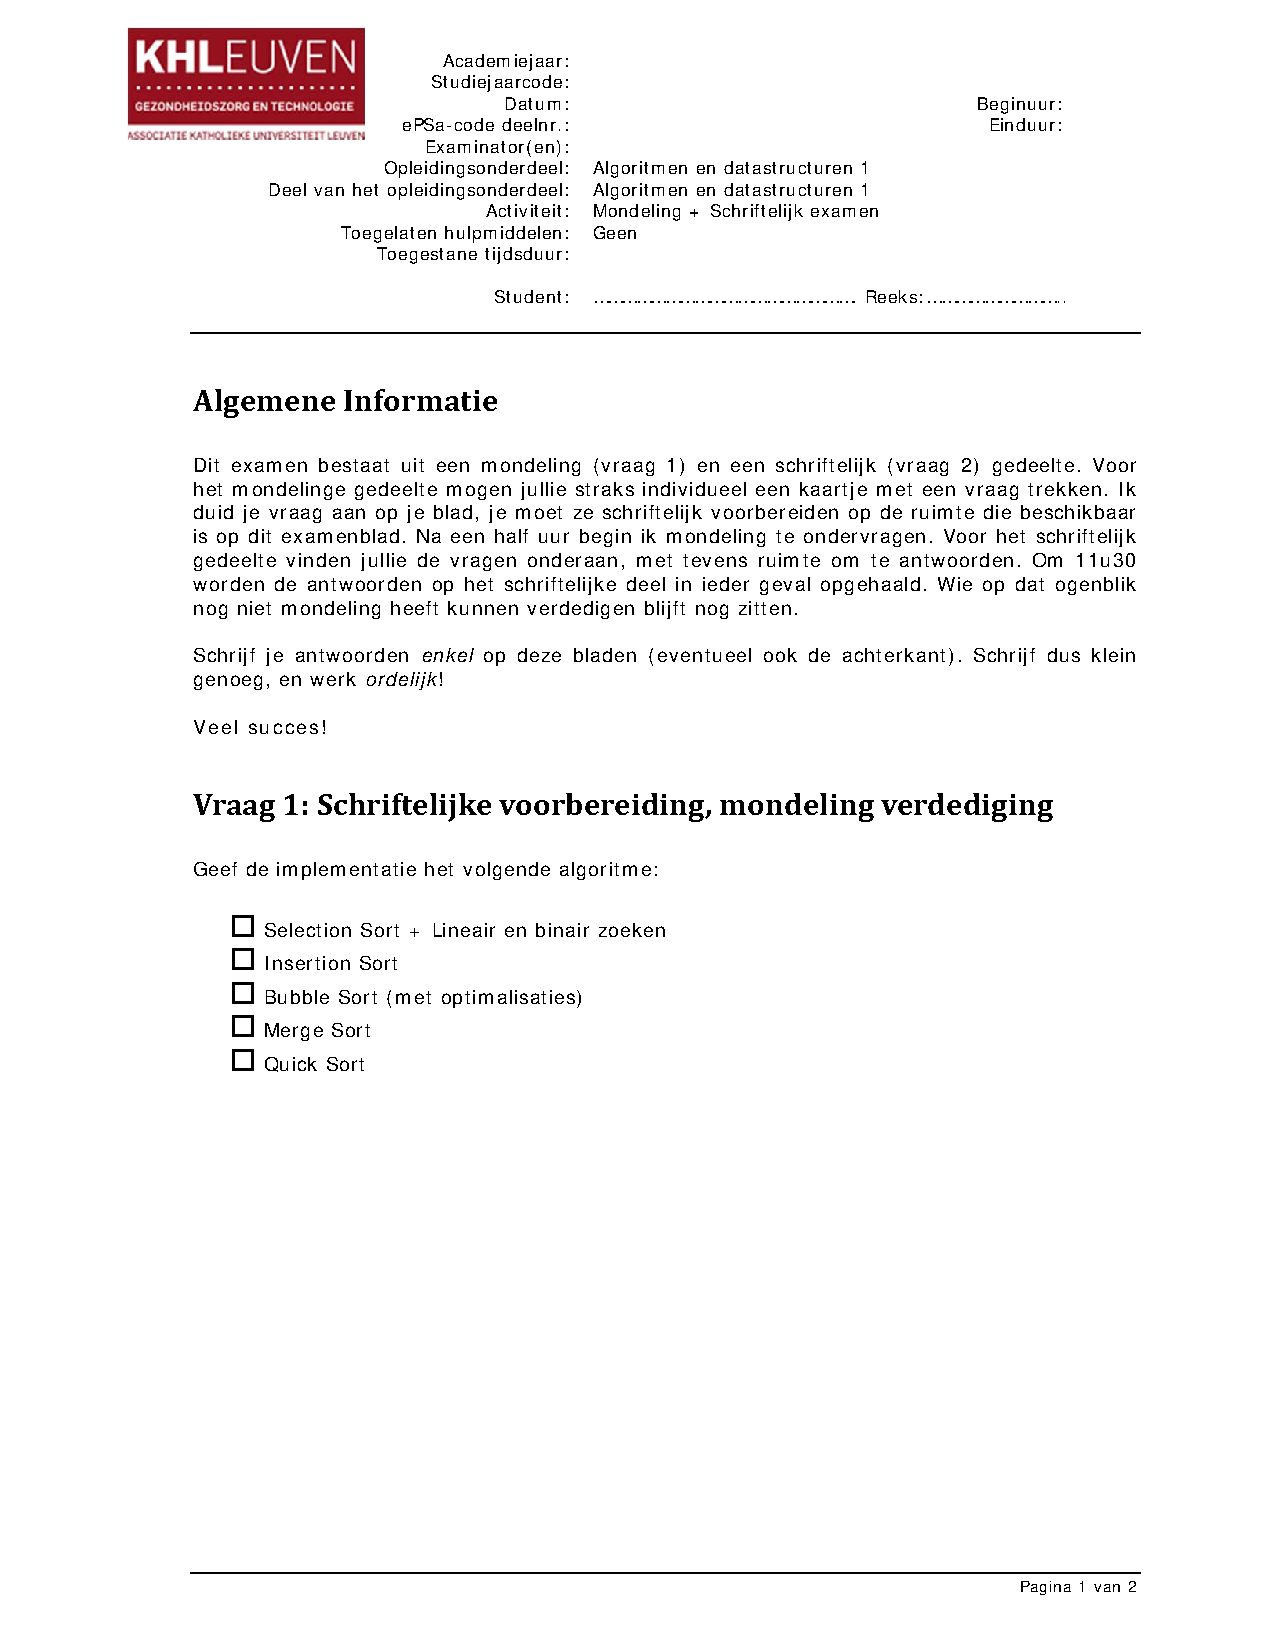
\includepdf[pages={-}]{Testen/Examen1.pdf}
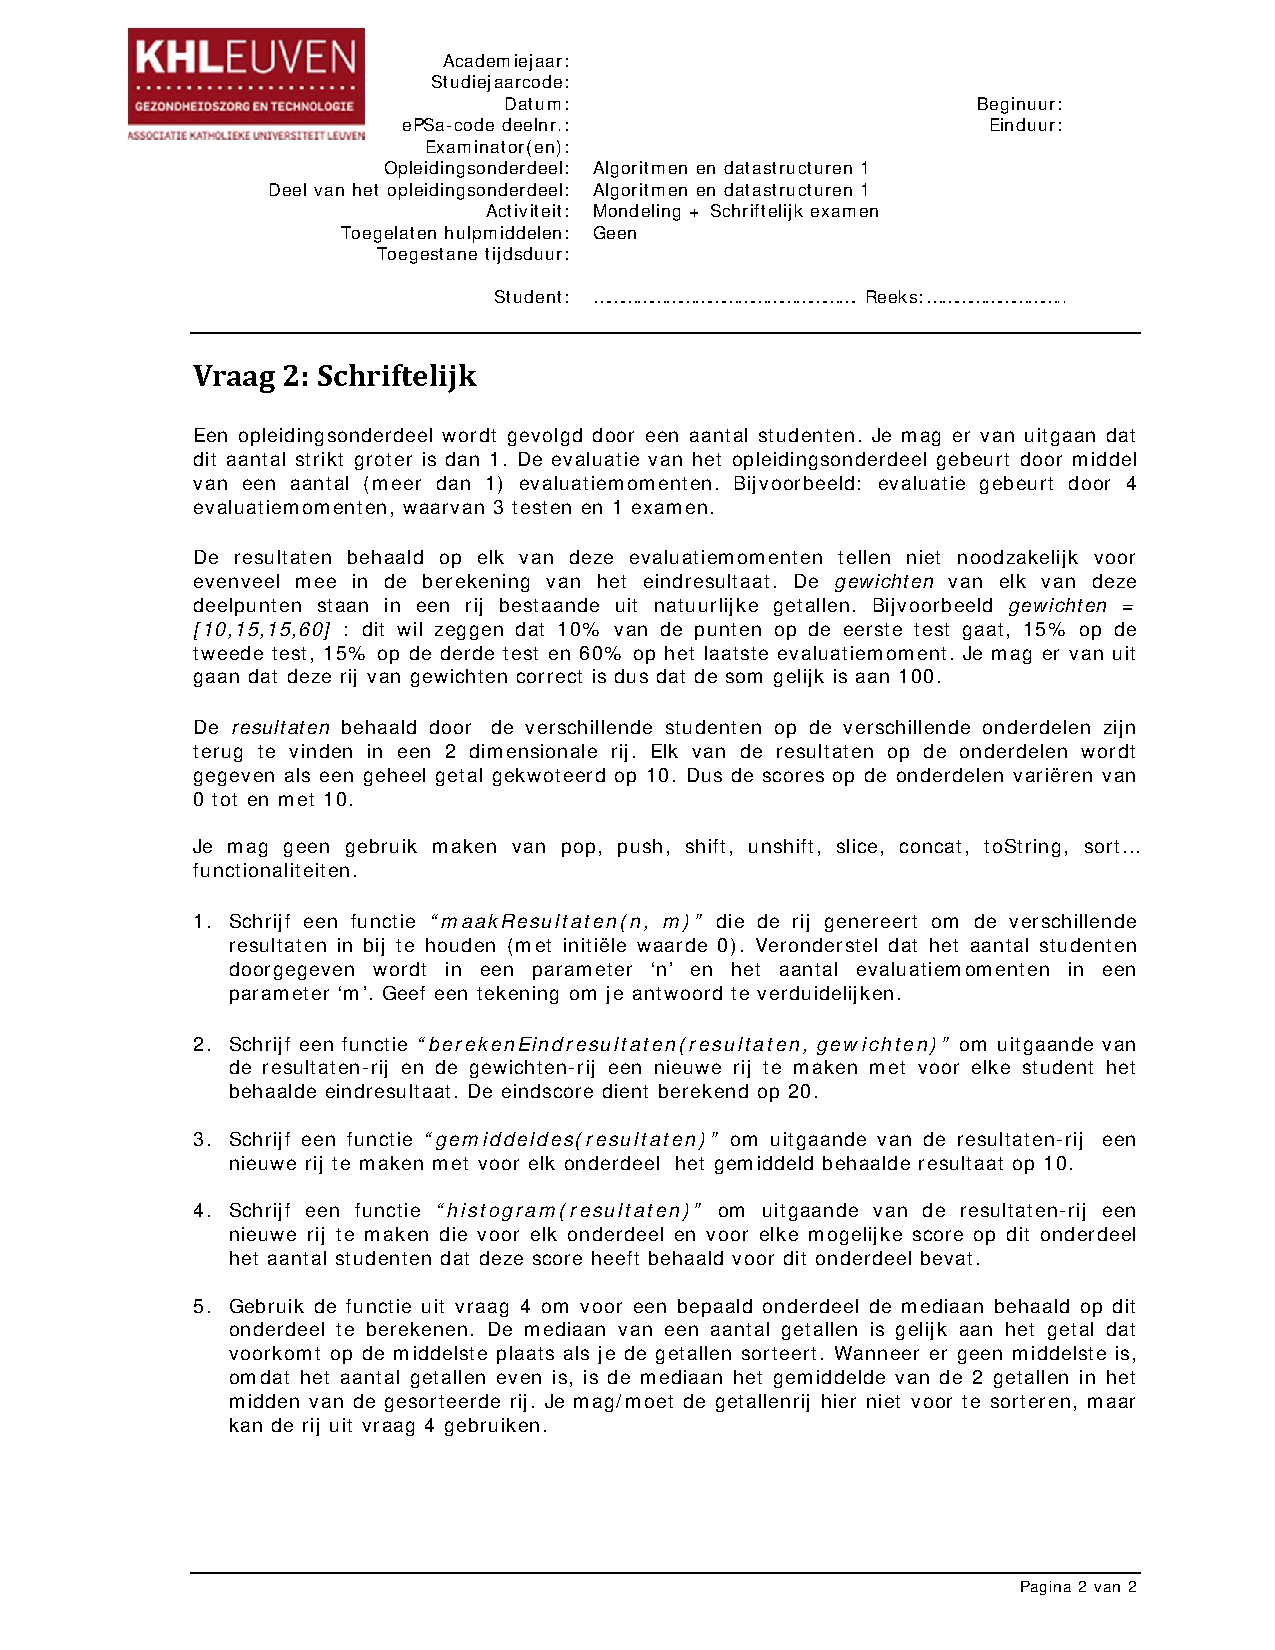
\includepdf[pages={-}]{Testen/Examen2.pdf}
